\chapter{Far field and near field}

An graphical illustration of the Far field and Near field \citep{farnear_field1}\citep{farnear_field2} can be seen on the following Figure:

\begin{figure}[H]
\centering
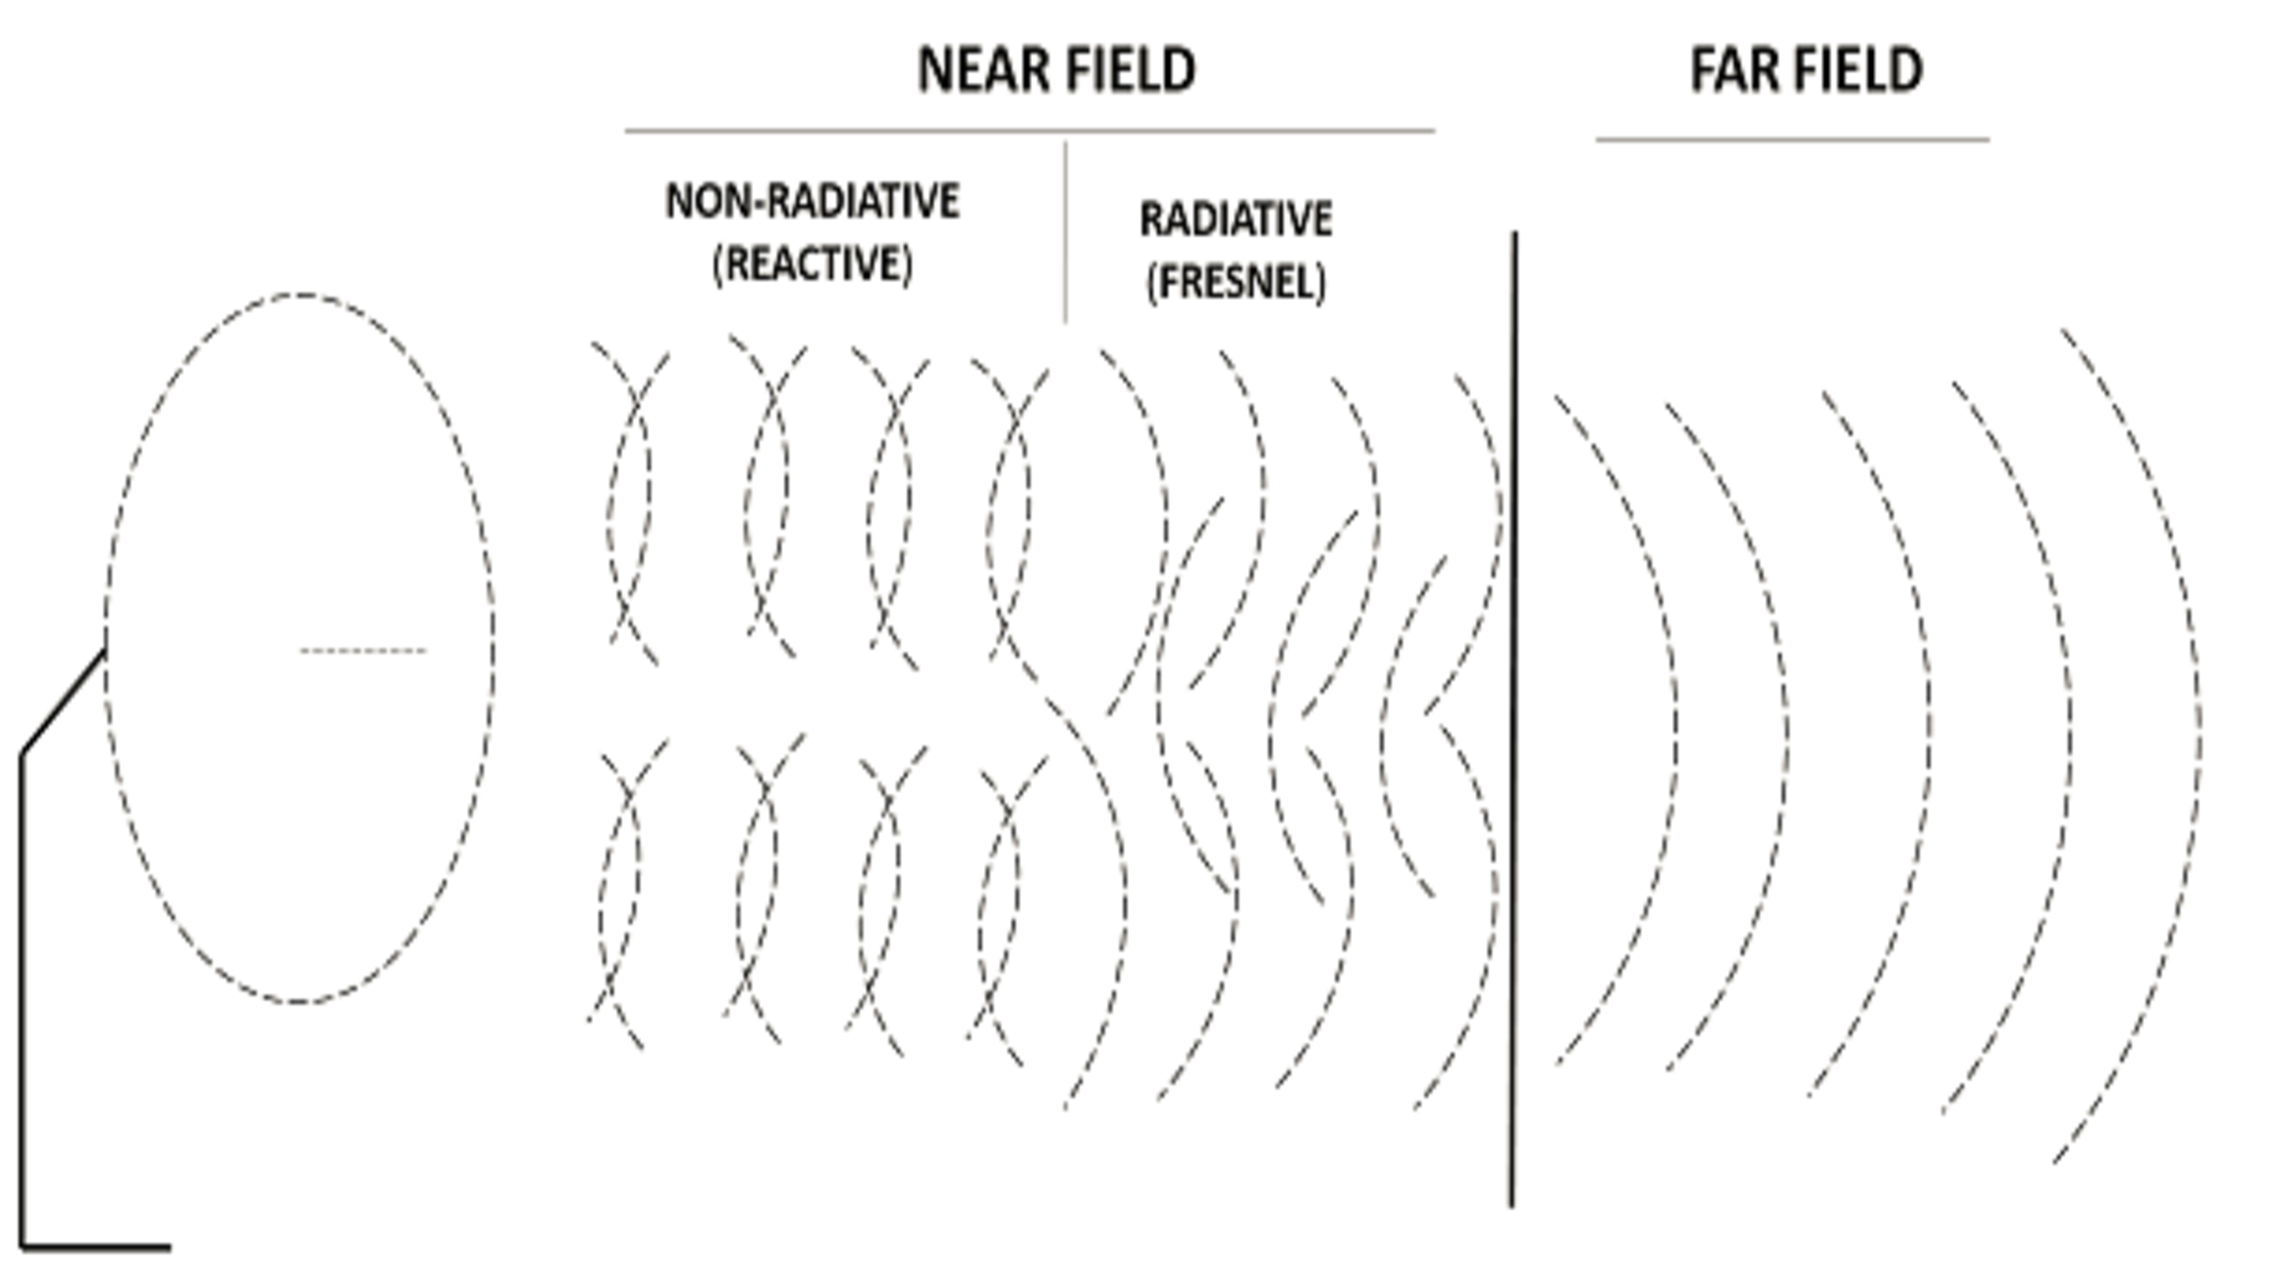
\includegraphics[width=0.6\textwidth]{nearfield_farfield.pdf}
\caption{Illustration of Near field and Far field \citep{farnear_field}}
\label{para_wave}
\end{figure}



\subsection{Far field region}

The Far field region is the region that is furthest from the antenna. The Far field region $R$ is given by the following formula:

\begin{equation}
R > \frac{2 \cdot D^{2}}{\lambda}
\label{far_field_eq1}
\end{equation}

\begin{where}
\va{$D$}{Is the maximum dimension of the antenna}{m}
\va{$\lambda$}{Wavelength}{m}
\end{where}

The Far field region $R$ provides the limit between Far field and Near field. The Far field region must also satisfy the following two equations:

\begin{align}
R &\gg D\\
R &\gg \lambda
\label{far_eq1_eq2}
\end{align}

The first two equations, ensure that the power radiated in a given direction from different parts of the antenna are approximately parallel. This helps to ensure that waves in the Far field behave like plane waves. Plane waves only radiate towards the forward direction, and are in parallel. %This is illustrated on the following Figure:

%\begin{figure}[H]
%\centering
%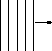
\includegraphics[width=0.2\textwidth]{para_wave.pdf}
%\caption{Illustration of Plane waves}
%\label{para_wave}
%\end{figure}

The third equation makes sure that the reactive Near fields are gone. The reactive near field is the region surrounding the antenna where the reactive field(standing waves or stored energy) are dominant. In a reactive field two oppositely waves are travelling, which are non-radiative, they do not radiate power, they store the energy. This means that the receiver antenna will not receive power in the Near field, as it does not radiate. %So the receiver antenna will not receive these standing waves, as a part of the power radiated, in the far field. 
The much larger sign $\gg$ stands for 10 times larger. 
%The problem with the reactive field is that the receiving and the transmitting antenna may interact with each other 




%%http://my.ece.msstate.edu/faculty/donohoe/ece3323antennas.pdf
%%http://www.antenna-theory.com/basics/fieldRegions.php
%% https://www.tutorialspoint.com/antenna_theory/antenna_theory_near_and_far_fields.htm

%Reactive Near fields are unwanted as they radiate back and forward  




%The Far field region starts approximately two wave lengths from the antenna and extends outwards. 


%In this region the radiation pattern does not change with the shape of the distance  


\subsection{Near field region}

In the Near field there are two regions the Non-radiative(Reactive) and Radiative(Fresnel) regions. The boundary for the Non-radiative(Reactive) is given in the following Equation:

\begin{equation}
R < 0.62 \cdot \sqrt{\frac{D^{3}}{\lambda}}
\label{far_field_eq1}
\end{equation}


While the Radiative(Fresnel) region is the region between the Near and Far fields. In this region unlike for the Far field region the shape of the radiation pattern may vary considerably with distance. The Radiative(Fresnel) region is given by the following Equation:


\begin{equation}
0.62 \cdot \frac{D^{3}}{\lambda} < R < \frac{2 \cdot D^{2}}{\lambda}
\label{far_field_eq1}
\end{equation}


The above can be summarized in the following Figure:

\begin{figure}[H]
\centering
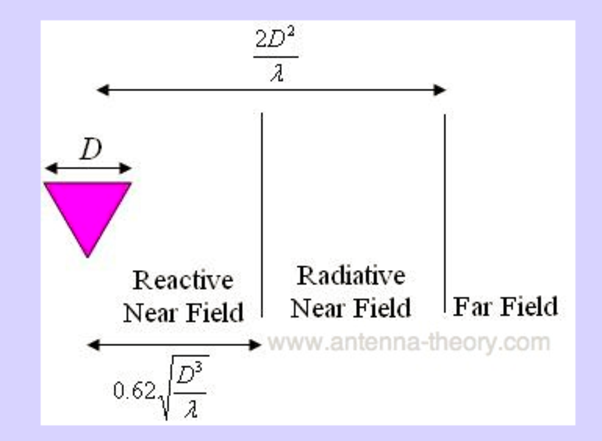
\includegraphics[width=0.5\textwidth]{nearfar_field_eq_ill.pdf}
\caption{Illustration of Near field and Far field \citep{farnear_field1}}
\label{nearfarf_eq_ill}
\end{figure}


\subsection{Far field calculation}

In order to calculate if the measurements are done in the Far field, the maximum dimension of a given antenna must be known. The maximum dimension $D$ is 0.105m. Then in terms of being in the Far field:

\begin{equation}
R > \frac{2 \cdot D^{2}}{\lambda}
\label{far_field_eq1}
\end{equation}



The wave length $\lambda$ for 868Mhz is given as:

\begin{equation}
\lambda = \frac{3E8 ms^{-1}}{0.868 Ghz} = 0.3453m
\end{equation}

Then:

\begin{equation}
R> \frac{2 \cdot (0.105m)^{2}}{0.3453m} = 0.0639 m 
\end{equation} 

While the minimum R is 1m, as the minimum distance between the transmitter and receiver antenna is 1 m. And as it can be seen 1m, the Far field equation is fulfilled. 